\documentclass[a4paper,12pt]{article}
\usepackage[utf8]{inputenc}
\usepackage[T2A]{fontenc}
\usepackage[russian,english]{babel}
\usepackage[pdftex]{graphics}
\DeclareGraphicsExtensions{.pdf,.png,.jpg}
\graphicspath{{pictures/}}
\begin{document}
\begin{center}
Санкт-Петербургский государственный политехнический университет
\\Кафедра компьютерных систем и программных технологий
\end{center}
\vspace*{10em plus .6em minus .5em}

\begin{center}
{\LARGEТелекоммуникационные технологии
\\Лабораторная работа №6
\\Цифровая модуляция}
\end{center}

\vspace*{5em plus .6em minus .5em}
\begin{flushright}
Выполнил:\\студент гр.33501/4\\Корсков Алексей\\Проверила:\\Богач Н.В.
\end{flushright}

\vspace*{15em plus .6em minus .5em}
\begin{center}
{\smallСанкт-Петербург
\\2018}
\end{center}
\pagestyle{empty}
\newpage
\pagestyle{plain}
{\bfseriesЦель}

Изучение методов модуляции цифровых сигналов.

{\bfseriesПостановка задачи}

\begin{itemize}
\item Получить сигналы BPSK, PSK, OQPSK, genQAM, MSK, MFSK
модуляторов
\item Построить их сигнальные созвездия
\item Провести сравнение изученных методов модуляции цифровых
сигналов
\end{itemize}

{\bfseriesТеоретическое обоснование}

Манипуляция (цифровая модуляция) — в теории передачи дискретных сообщений процесс преобразования последовательности кодовых символов в последовательность сигналов (частный случай модуляции — при дискретных уровнях модулирующего сигнала).

В зависимости от изменяемых параметров манипуляцию разделяют на амплитудную, фазовую, частотную и квадратурную.

При \textbf{частотной манипуляции} (ЧМн; английский термин - frequency shift keying,\textbf{FSK}) вид манипуляции, при которой скачкообразно изменяется частота несущего сигнала в зависимости от значений символов информационной последовательности. Частотная манипуляция весьма помехоустойчива, поскольку помехи искажают в основном амплитуду, а не частоту сигнала.

\textbf{MSK} (minimum shift key) - \textbf{манипуляция с минимальным сдвигом частоты.} Разность частот сигналов, соответствующих различным битам, равна половине скорости передачи информации. Манипуляция называется с минимальным сдвигом частоты, так как значение $\Delta f = \frac{1}{2T}$ является минимальной разностью частот, при котором сигналы с различными частотами, являются ортогональными. 

\textbf{MFSK} - \textbf{Многопозиционная частотная манипуляция.} Метод манипуляции, при котором N дискретных состояних входного сигнала преобразуются в набор из N фиксированных частот, передаваемых параллельно или последовательно.

\textbf{Амплитудная манипуляция} (АМн; английский термин - amplitude shift keying, \textbf{ASK}), при которой скачкообразно меняется амплитуда несущего колебания, является частным случаем квадратурной манипуляции.

\textbf{Фазовая манипуляция} (ФМн; английский термин - phase shift keying, \textbf{PSK}), при которой скачкообразно меняется фаза несущего колебания, тоже является частным случаем квадратурной манипуляции.
\newpage

{\LargeХод работы}
\begin{enumerate}
{\itemСигнальное созвездие BPSK
\center{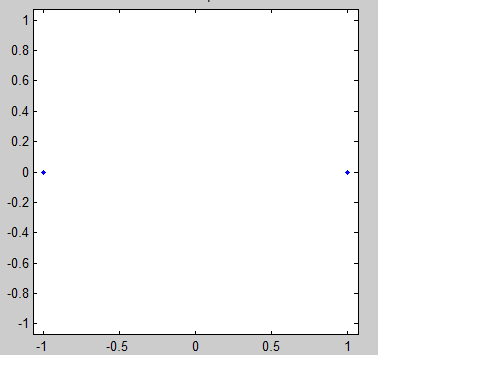
\includegraphics{./pictures/pic1.png} \\ Рис.1 Сигнальное созвездие BPSK}
\\}

{\itemСигнальное созвездие PSK
\center{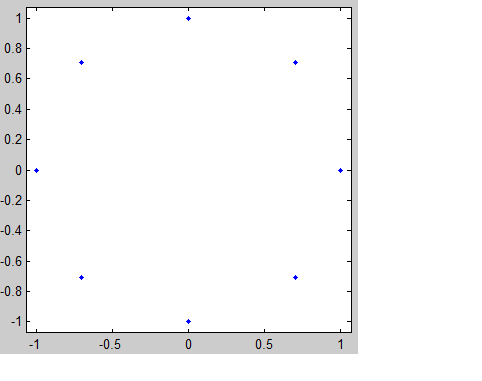
\includegraphics{./pictures/pic2.png} \\ Рис.2 Сигнальное созвездие PSK}
\\}

{\itemСигнальное созвездие OQPSK
\center{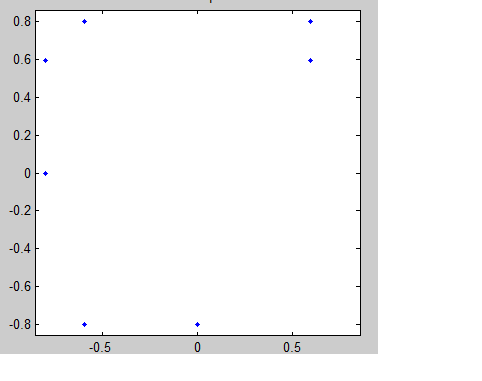
\includegraphics{./pictures/pic3.png} \\ Рис.3 Сигнальное созвездие OQPSK}
\\}

{\itemСигнальное созвездие genQAM
\center{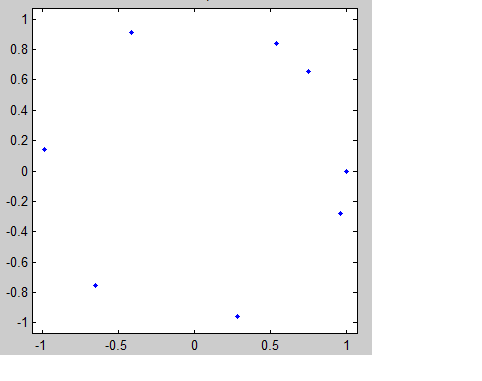
\includegraphics{./pictures/pic4.png} \\ Рис.4 Сигнальное созвездие genQAM}
\\}

{\itemСигнальное созвездие MSK
\center{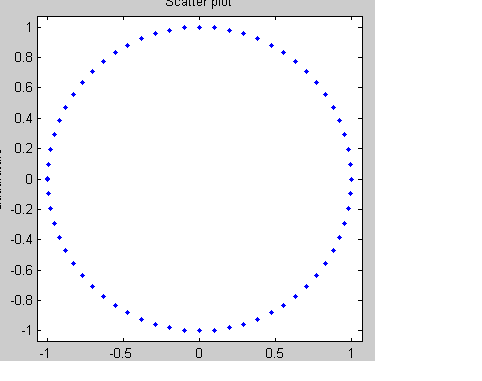
\includegraphics{./pictures/pic5.png} \\ Рис.5 Сигнальное созвездие MSK}
\\}

{\itemСигнальное созвездие FSK
\center{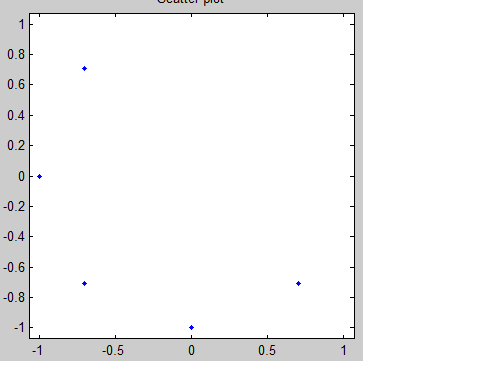
\includegraphics{./pictures/pic6.png} \\ Рис.6 Сигнальное созвездие FSK}
\\}

{\bfseries\LARGEВывод}

В технике цифровой связи методы модуляции играют весьма значительную роль. Помимо своей основной функции – преобразования символ – сигнал – процесс модуляции является составной частью общего процесса согласования сигнала с характеристиками канала.

Применение многопозиционной QAM способствует передаче большего количества информации, однако в реальных усло­виях, при наличии помех, на приемной стороне возможно ошибочное определение амплитуды и фазы передаваемого сигнала. Это обстоя­тельство и ограничивает количество информации, передаваемое од­ним символом. Тем не менее, основное преимущество QAM перед другими видами модуляции — в ее хорошей помехозащищенности. 

Способ модуляции PSK применяется в случаях, когда необхо­димо сохранить постоянной амплитуду передаваемого сигнала или исключить амплитуду из числа параметров, изменяемых в процессе модуляции. 
\end{enumerate}
\end{document}
